\documentclass[12pt]{article}
% Load packages
\usepackage{times}
\usepackage{cite}              % Make references as [1-4], not [1,2,3,4]
\usepackage{wrapfig}
\usepackage[super]{natbib}
\usepackage{url}                % Formatting web addresses
\usepackage{ifthen}             % Conditional
\usepackage{multicol}                   % Multi-column pages
\usepackage[utf8]{inputenc}     % Unicode support
\usepackage{amsmath}           % Support for writing math formulas
\usepackage{amssymb}           % Support for writing math formulas
\usepackage{epsfig}            % Support separate PostScript files for Fig.s
\usepackage{epstopdf}                   % Converts eps Fig.s to pdf
\usepackage{graphicx}                   % Graphics functions
\usepackage[margin=0.1pt,font=footnotesize,labelfont=bf]{caption}
\usepackage{setspace}                   % Provides line spacing environments
\usepackage{colortbl}
\usepackage[wide]{sidecap}              % Can typeset caption aside the Fig., allows use of margin for Fig.s wider than \textwidth.
\usepackage{supertabular}               % Tables spanning multiple pages
\usepackage{comment}
\usepackage{lineno}
\urlstyle{rm}                                   % URL style
\usepackage{float}
\usepackage[FIGTOPCAP,nooneline]{subfigure}
\captionsetup{font={footnotesize},aboveskip=0pt}        % Styles Fig. captions
\usepackage[letterpaper,bindingoffset=0.0in,left=1.0in,right=1.0in,top=1.0in,bottom=1.0in,footskip=.25in]{geometry}
\usepackage[font=scriptsize,labelfont=bf]{caption}
\usepackage{blindtext}
\date{}
\usepackage{psfrag}
\usepackage{anyfontsize}
% \doublespacing
\singlespacing
\frenchspacing     % Eliminates double spaces between sentences
\usepackage{titlesec}
\titleformat{\section}
  {\normalfont\bfseries}{\thesection}{1em}{}
\titleformat{\subsection}[runin]
  {\normalfont\itshape}{\thesubsection}{1em}{}
\titleformat{\subsubsection}[runin]
  {\normalfont\itshape}{\thesubsubsection}{1em}{}
\titlespacing*{\section}{0pt}{*1.5}{8pt}
\titlespacing*{\subsection}{0pt}{*1.5}{8pt}
\titlespacing*{\subsubsection}{0pt}{*1.5}{8pt}
\newboolean{publ}
%Publication style settings
%\newenvironment{bmcformat}{\fussy\setboolean{publ}{true}}{\fussy}
\renewcommand{\rmdefault}{ptm}\renewcommand{\sfdefault}{ptm}
\renewcommand{\bibnumfmt}[1]{#1.}    % Change the number format in the ref list
%\renewcommand{\Fig.name}{Fig..}     % Change Fig. to Fig..

%for supplimental material
\newcommand{\beginsupplement}{%
        \setcounter{table}{0}
        \renewcommand{\thetable}{S\arabic{table}}%
        \setcounter{figure}{0}
        \renewcommand{\thefigure}{S\arabic{figure}}%
     }
%%%%%%%%%%%%%%%%%%%%%%%%%%%%%%%%%%%%%%%%%%%%%%%%%%%%%%%%%%%%%%%%%%%%%
%%%%%%%%%%%%%%%%%%%%%%%%%%%%%%%%%%%%%%%%%%%%%%%%%%%%%%%%%%%%%%%%%%%%%
\everymath{\displaystyle}
\begin{document}
%%%%%%%%%%%%%%%%%%%%%%%%%%%%%%%%%%%%%%%%%%%%%%%%%%%%%%%%%%%%%%%%%%%%%
% TITLE PAGE
%%%%%%%%%%%%%%%%%%%%%%%%%%%%%%%%%%%%%%%%%%%%%%%%%%%%%%%%%%%%%%%%%%%%%
\begin{titlepage}
  \begin{center}
    \vspace*{\stretch{0.8}}
    {\LARGE{Towards a Personalized, State Aware Model of Trauma}}\par
    \vspace{5em}
    { \Large{Rachel LeCover} \\
    \vspace{1em}
    { \large{Advisor: Jeffrey D. Varner}}\par   
     \vspace{3em}
    { \large{Qualifying Examination}}\par
     \vspace{1em}
    { \large{August 1, 2016}}\par
    \begin{figure}[h]
    \vspace{3em}
       \centering
       
\includegraphics[width=0.7\textwidth]{figures/CULogo187}
       \end{figure}
    \vspace{2em} \large{ \textit{School of Chemical and Biomolecular Engineering \\ \vspace{0.5em} Cornell University, Ithaca, NY}}}\par
    \vspace{3em}
  \end{center}
\end{titlepage}
\pagebreak
%%%%%%%%%%%%%%%%%%%%%%%%%%%%%%%%%%%%%%%%%%%%%%%%%%%%%%%%%%%%%%%%%%%%%
% INTRODUCTION
%%%%%%%%%%%%%%%%%%%%%%%%%%%%%%%%%%%%%%%%%%%%%%%%%%%%%%%%%%%%%%%%%%%%%
\setcounter{page}{1}
\section*{Abstract}
We propose the development of a personalized, state aware, high fidelity model of traumatic injury. The proposed model will capture both the physical and biochemical aspects of trauma. We have constructed an eight compartment body, with a small wound connected to the arterial compartment. Through a heart rate prediction model, we allowed the volumes of compartments to change based on the concentration of vasoactive factors. Future work will include incorporating more physiological functions into the model as well as personalization.
\section*{Introduction} 
\subsection*{Motivation} Coagulopathy, a disorder impairing the ability of blood to clot, is one of the three legs of the ``lethal triad", a set of conditions commonly seen in trauma patients. These conditions feedback on each other, worsening the patient's chance at survival. About a quarter of trauma patients suffer from coagulopathy, and the irreversible bleeding that follows majorly contributes to mortality from trauma. \cite{kauvar2006impact} Trauma patients who have normal prothrombin times (PT) and partial thromboplastin times (PTT) upon hospital arrival have much greater odds of survival than patients who are suffering from coagulopathy and have abnormal PT or PTT. \cite{macleod2003early} Additionally, patients with coagulopathy but the same Injury Severity Score (ISS) as patients without coagulopathy were more likely to die. \cite{brohi2003acute} Furthermore, the greater the degree of coagulopathy, the higher the mortality rate. \cite{frith2010definition}
For those in the military, hemorrhage is the cause of nearly 90\% of potentially survivable deaths. \cite{blackbourne2010decreasing} This exsanguination can lead to a dilution of coagulation factors in the blood, resulting coagulopathy.
At the present, there are no universal guidelines on which fluids an exsanguinating patient should receive and at what ratio. North American hospitals give patients suffering from major hemorrhage fresh frozen plasma, whereas European hospitals would give these patients clotting factor concentrates.\cite{hunt2014bleeding} 
In other cases, severe trauma can lead to disseminated intravascular coagulation (DIC), when the balance shifts and the patient's blood becomes overly prone to clotting. \cite{boccaccio1981disseminated} Treatment for disseminated intravascular coagulation is heparin, and possibly platelets.\cite{stacca1989disseminated} Patients suffering from DIC have a much higher mortality rate than other trauma patients. \cite{gando2001disseminated}
\begin{wrapfigure}{R}{7cm}
                \vspace{-20pt}
        \centering
        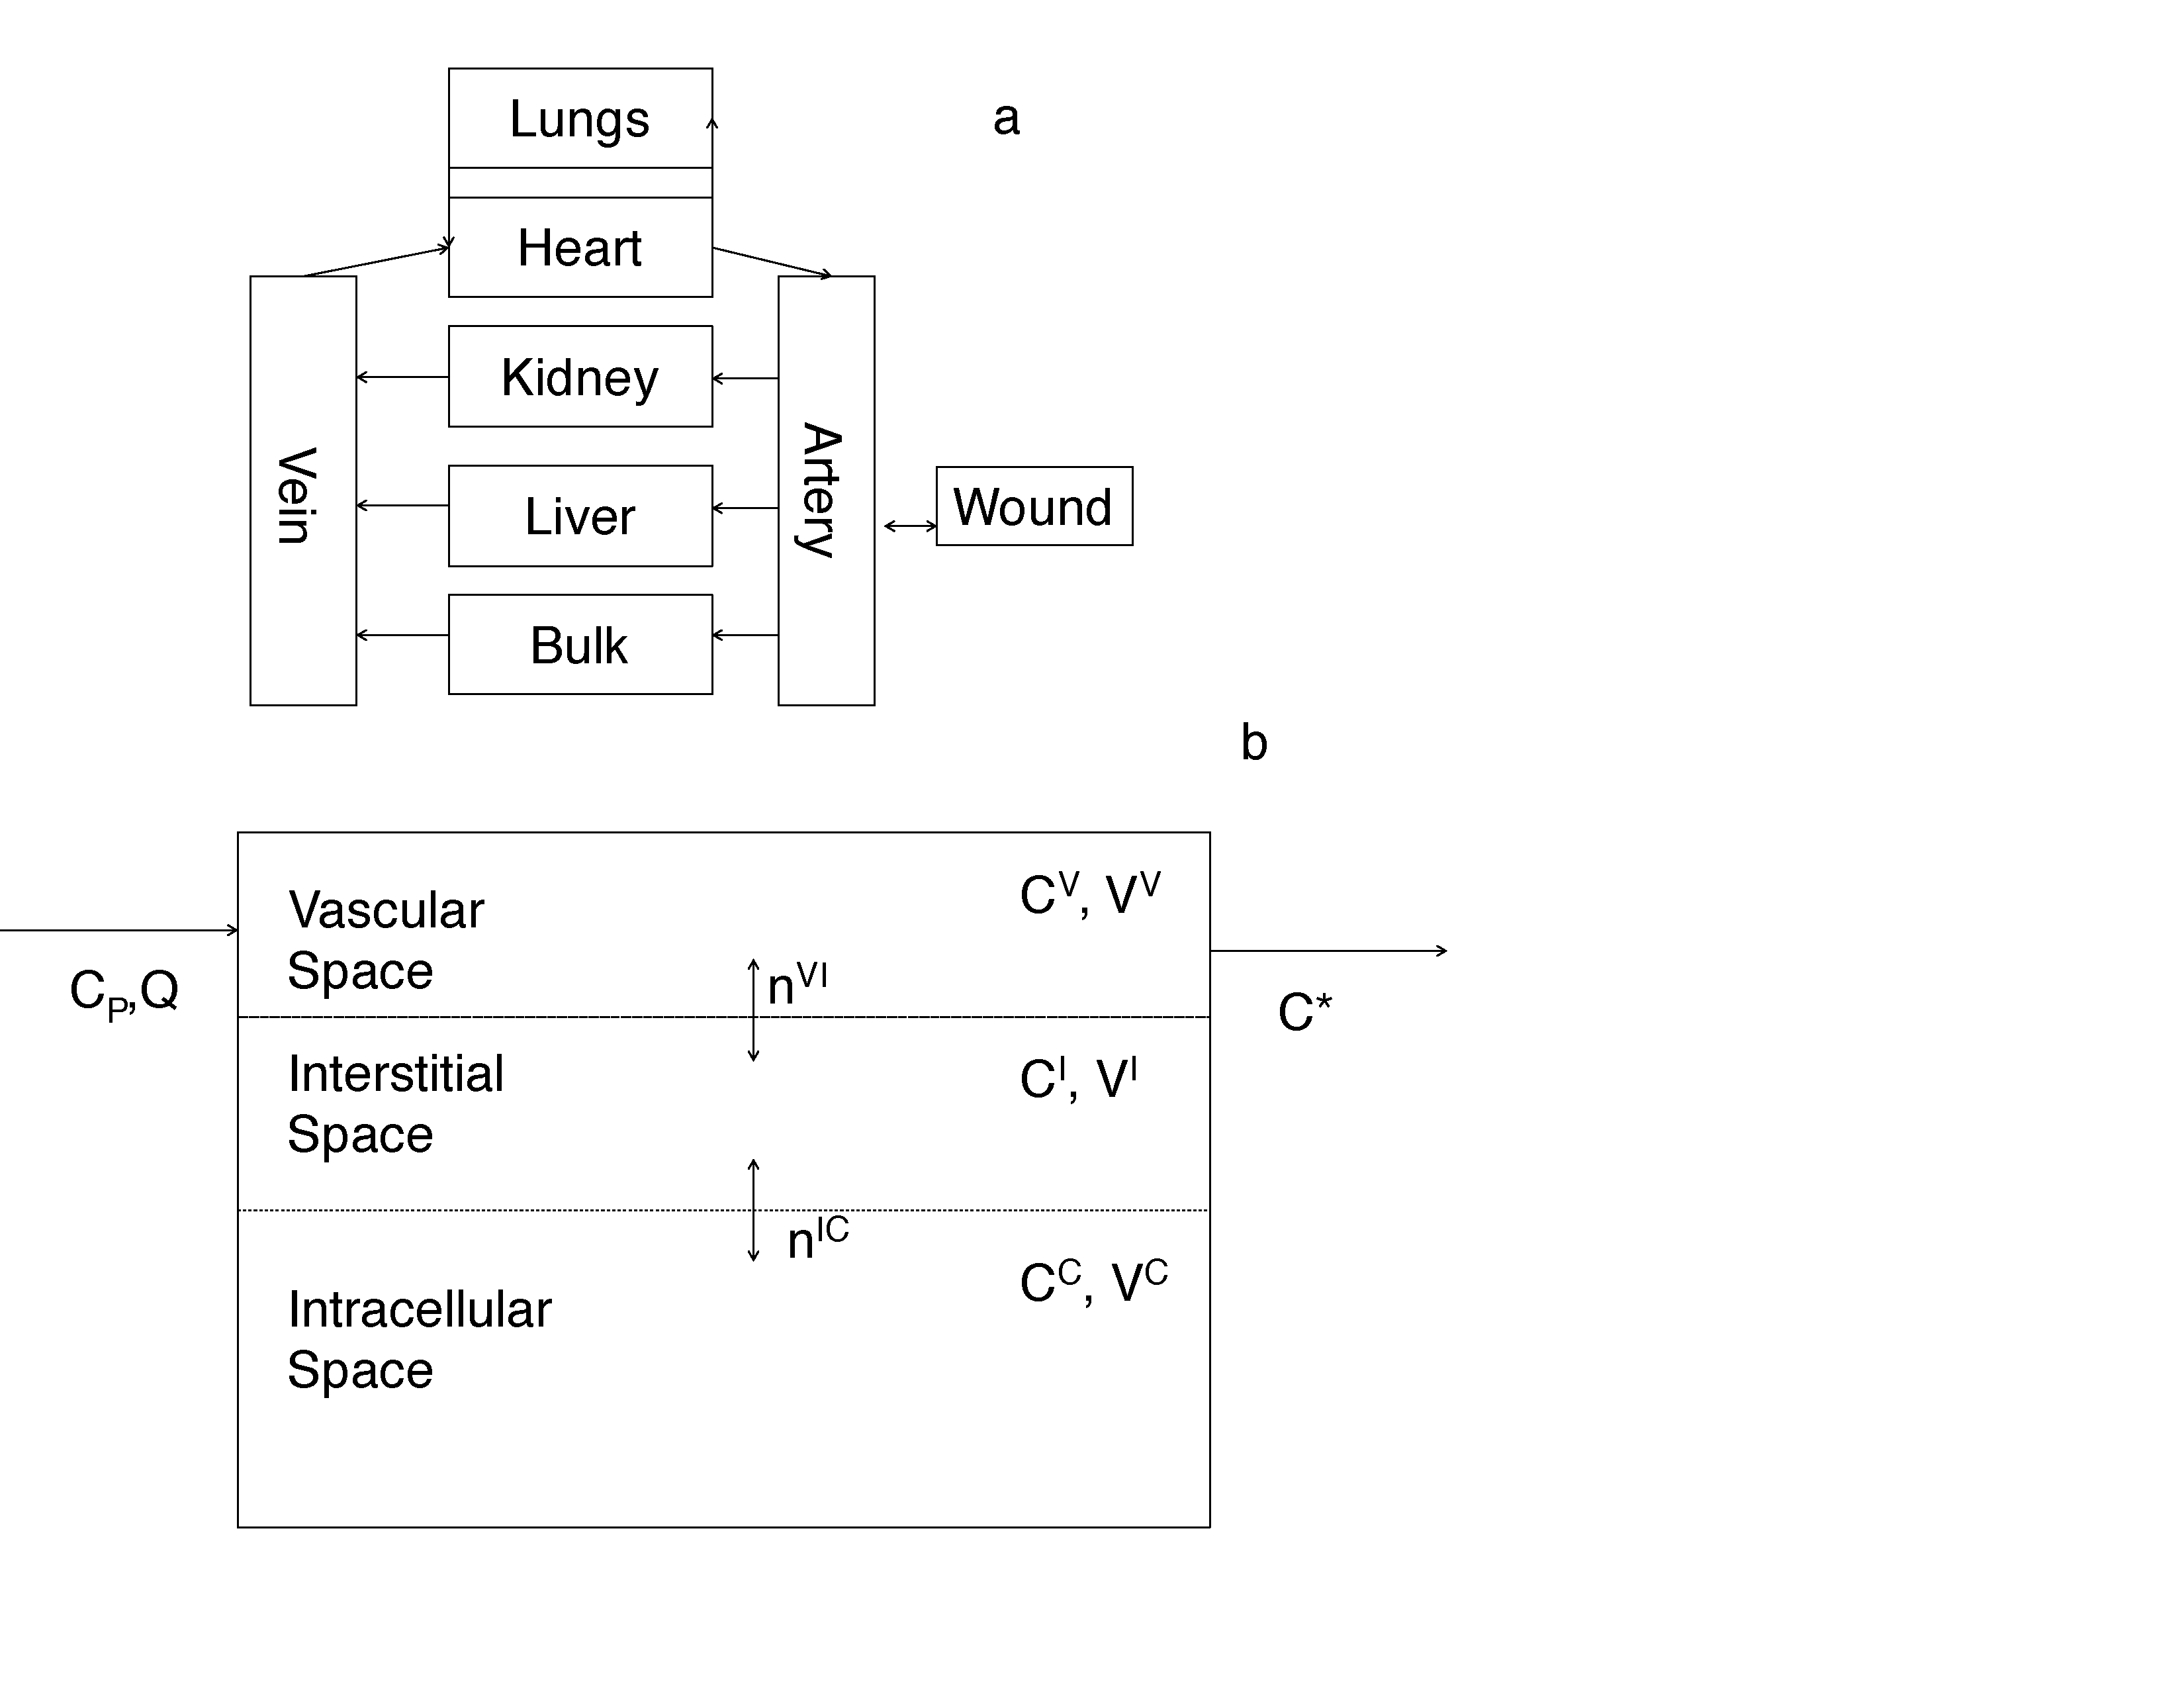
\includegraphics[height=10cm]{figures/bothbodyfigures}
         \vspace{-20pt}
        \caption{\scriptsize Figure a shows a eight compartment PBPK, with arterial and venous blood pools, with a wound off of the aerial blood pool. Figure b shows a sample organ broken up into subcompartments.}
                 \label{fig:SamplePBPK}
\end{wrapfigure} 
 
\subsection*{Research aims:} The goals of my research are to produce a state-aware model of trauma that can be used as a predictive tool by medical professionals. This tool may be used to predict survival rates and the interventions necessary to reduce mortality of trauma patients. Additionally, this model can be used to simulate interventions to provide clinical treatment recommendations.
%%%%%%%%%%%%%%%%%%%%%%%%%%%%%%%%%%%%%%%%%%%%%%%%%%%%%%%%%%%%%%%%%%%%%
% SIGNIFICANT PREVIOUS WORK
%%%%%%%%%%%%%%%%%%%%%%%%%%%%%%%%%%%%%%%%%%%%%%%%%%%%%%%%%%%%%%%%%%%%%
\section*{Significant Previous Work}
\subsection*{Physiologically Based Pharmoacokinetic Models}
Physiologically based pharmacokentic models, abbreviated as PBPKs, are commonly used to model how substances distribute in living systems, such as the human body. PBPK modeling divides the system of interest into several (generally assumed to be well mixed) compartments, with specified flow rates between each compartment and pools of venious and arterial blood. A simple diagram of a PBPK is shown in Figure \ref{fig:SamplePBPK}. 
   
We can then write mass balances over each compartment and one over the entire system and solve them to describe the distribution of the substance of interest over time. 
In some cases, each compartment is broken into subcompartments to create a more accurate model, as shown in Figure \ref{fig:SamplePBPK}.
We then write mass balances over the various compartments of the $i^{th}$ organ. 
\begin{equation}
V^V_i\frac{dC^V_i}{dt} = Q_iC_p-Q_iC_i^V-n_i^{V-I}
\end{equation}
\begin{equation}
V^I_i\frac{dC^I_i}{dt} =n_i^{V-I}-n_i^{V-C}
\end{equation}
\begin{equation}
V^C_i\frac{dC^C_i}{dt} =n_i^{I-C}
\end{equation}
The superscript V denotes vascular, I interstitial, P plasma, and C cellular, $n_i$ describes the flux between compartments, $Q_i$ gives the flow rate between compartments, and $C_i$ is the concentration in the $i^{th}$ compartment. \citep{clewell2007physiologically} The volumes of the compartments are assumed to be constant, so dilution terms are neglected.
\subsection*{Models of Coagulation and Fibrinolysis}
Historically, the coagulation cascade was considered to be two distinct pathways, the extrinsic and intrinsic, but today, it is known that the two pathways are linked.\cite{adams2009review} 
\subsubsection*{Clot Formation}
The coagulation process begins when an injury occurs, which exposes tissue factor, a transmembrane protein expressed on the surface of cells surrounding blood vessels. \citep{mackman2009role} The newly exposed tissue factor can then bind to factor VIIa (FVIIa), thus forming the extrinsic tenase complex. The tenase complex catalyzes the conversion of FX and FIX to their active forms, FXa and FIXa. \cite{mann2006models} FXa converts a small amount of prothrombin to thrombin. \cite{orfeo2004factor} This thrombin then activates FV, FVIII, and FXIII giving rise to FVa, FVIIIa, FXIIIa. Thrombin also binds to G-coupled protein receptors on platelet membranes, activating the platelets and inducing them to aggregate.\citep{hoffman2009hematology} FIXa and FVIIa form the intrinsic factor tenase complex, which strongly converts FX to FXa, leading to a large increase in thrombin production. FXa and FVa bind together to form the prothrombinase complex, which converts prothrombin to thrombin about $10^8$ times efficiently as FXa alone. \cite{walker1994activation} The large amount of thrombin produced leads to the conversion of fibrogen to fibrin, and FXIIIa helps cross link the fibrin to form a stable network, leading to the formation of a clot. \cite{hoffman2009hematology}

This process has been modeled in great detail using ordinary differential equations, keeping track of 92 proteins and 148 protein-protein interactions. \cite{luan2007computationally} Wajima et al modeled coagulation as well as the effects of wafarin, vitamin K, and unfractionated heparin.\cite{wajima2009comprehensive} Additionally, it has been modeled as a set of positive feedback loops, with the last loop further activating the first loop. \cite{beltrami1995mathematical} Zarnitsina et al considered the biology of coagulation in great detail to to model clot growth. \cite{zarnitsina1996mathematical} They compared their model to data collected at varying concentrations of calcium, and found good agreement. More recently, Varner et al created a reduced order model of coagulation by combining ordinary differential equations with logical rules. \cite{sagar2015dynamic} This reduced order model contains only five differential equations, making it much less computationally intensive to solve. 
\subsubsection*{Clotting Regulation}
The clot formation process, with respect to thrombin, is a positive feedback loop with a small amount of thrombin leading to the generation of large amounts. This process can be stopped by several different inhibitors: tissue factor pathway inhibitor (TFPI), antithrombin, protein C, and protein Z.  
Tissue factor pathway inhibitor stops the clotting process in two ways: it binds to the FVIIa:TF complex, making it unavailable to produce FXa and FIXa, and it binds to already produced FXa, rendering it inactive. \cite{lwaleed2006tissue} Antithrombin binds to active factors, preventing them from further catalyzing the clotting process. \cite{olson1994regulation} Protein C, with its cofactor protein S, inactivates factors Va and VIIIa. \citep{esmon1987anticoagulation} Protein Z complexes with protein Z-dependent protease inhibitor in plasma, and reduces the activity of FXa, FXIa, and FIXa. \citep {corral2007protein}
Thrombin activated fibrinolysis inhibitor (TAFI) is activated the thrombomodulin-thrombin complex. \citep{chapin2015fibrinolysis}. It removes the lysine and arginine residues form the C-terminal of fibrin, which reduces the number of sites at which plasmiogen can bind, stabilizing the clot. 
\subsection*{Fibrinolysis}
Fibrinolysis acts to break down clots. If it and coagulation are not balanced, coagulopathy or disseminated intravascular coagulation may occur. The enzyme that breaks down clots, plasmin, has two activators, tPA and uPA. \cite{wiman1978molecular} Plasminogen is converted to plasmin through the actions of tissue plasmiogen activator (tPA) or urokinase (uPA) on the surface of the clot or on cell membranes. \citep{chapin2015fibrinolysis} Both tPA and uPA are serine proteases and have short half-lives in circulation, on the order of 4-8 minutes. They are destroyed in the liver. Their locations of manufacture differ: tPA is produced endothelial cells, uPA is produced by monocytes and macrophages. Both are inhibited by plasmiogen activator inhibitor-1 (PAI-1). tPA increases dramatically in activity when it binds fibrin. \citep{chapin2015fibrinolysis}
Bannish created a very detailed model of fibrinolysis using a stochastic model to model tPA binding and combined that with a macrosccale model to measure how fast the lysis front moves. \cite{bannish2012modelling} The dissolution of clots has also been modeled using the Naiver Stokes equation for flow over and through the clots combined with mass balances over the relevant species.\cite{wootton2002experimental} 
\subsection*{Previous Trauma Models}
Several whole body models of trauma exist, however, they tend to either simplify the body or the coagulation process. 
Ho et al developed a model that considered blood to be two distinct parts, either hematocrit or plasma, and assumed that the rate of fluid loss was the same as the rate as fluid replacement. They did not model any of the dynamics of the coagulation process, rather, they lumped all of the coagulation factors into one variable, which they correlated with prothromin time. \cite{ho2005mathematical} Their model provides guidance on the ratio of fresh frozen plasma (FFP) to packed red blood cells (PRBC) that patients with excessive blood loss should receive. 
Hirshberg et al modeled blood as having three compartments: red cells, plasma, and water, and allowed flow between these compartments based on systolic blood pressure. \cite{hirshberg2003minimizing} They used prothrombin time to quantify if a patient was at risk for dilutional coagulopathy, and did not consider the biological mechanisms behind coagulation.
Simpson et simulated the first two hours of hemorrhage by modeling blood pressure as a function of blood loss.\cite{simpson1996computer} This model predicts hematocrit levels over time, but not the levels of specific proteins. 
Reisner et al re-purposed their model of the cardiovascular system (which was originally created to predict how the cardiovascular system responds to orthostatic stress) to study hemodynamic responses to hemorrhage.\cite{reisner2013computational} Their model includes the heart and pulmonary circulation as well as four peripheral tissue compartments representing the upper body, legs, viscera and kidneys, each of which received the same fraction of the cardiac output. They modeled blood by separating it into two components: red blood cells and plasma. This model includes transcapillary fluid exchange and lymphatic flow, but groups all proteins together. 
%%%%%%%%%%%%%%%%%%%%%%%%%%%%%%%%%%%%%%%%%%%%%%%%%%%%%%%%%%%%%%%%%%%%%
% PRELIMINARY RESULTS
%%%%%%%%%%%%%%%%%%%%%%%%%%%%%%%%%%%%%%%%%%%%%%%%%%%%%%%%%%%%%%%%%%%%%
\section*{Preliminary Results}
\subsection*{Incorporating Reduced Order Model into PBPK}
We have constructed an eight compartment model of the human body, using the Kwatee code generation system. In this model, blood flows from a venous pool, to the heart, through the lungs, back through the heart, an into an arterial blood pool. Blood then passes from the arteries through the liver, kidney, or bulk to the veins. All of the proteins flow freely between compartments, except for thrombomodulin and trigger (a stand in for tissue factor), which are bound to cell membranes.\cite{esmon1989roles} We simulated a small wound being present to the arterial blood pool, with a volume of .5\% of the total blood volume. Figure \ref{fig:SamplePBPK}a shows the layout of the simulated body. We modeled the dynamics of coagulation in each compartment using the reduced order model previously mentioned, as shown in Figure \ref{fig:comparsionoftrigger}. Changing the concentration of trigger, which biologically corresponds to tissue factor, in the wound compartment dramatically changes the thrombin peak in the wound (second row, right), but only slightly shifts the thrombin peaks in the other compartments. The higher trigger concentrations lead to faster activation of protein C in other compartments, as shown in the third row. Presently, this model has no protein synthesis, something that may be included in future models. The patient is bleeding out at a constant rate of 10.5 mL/min, which would lead to complete exsanguination in a bit less than ten hours.
\begin{figure}
%\begin{wrapfigure}{R}{\textwidth}
        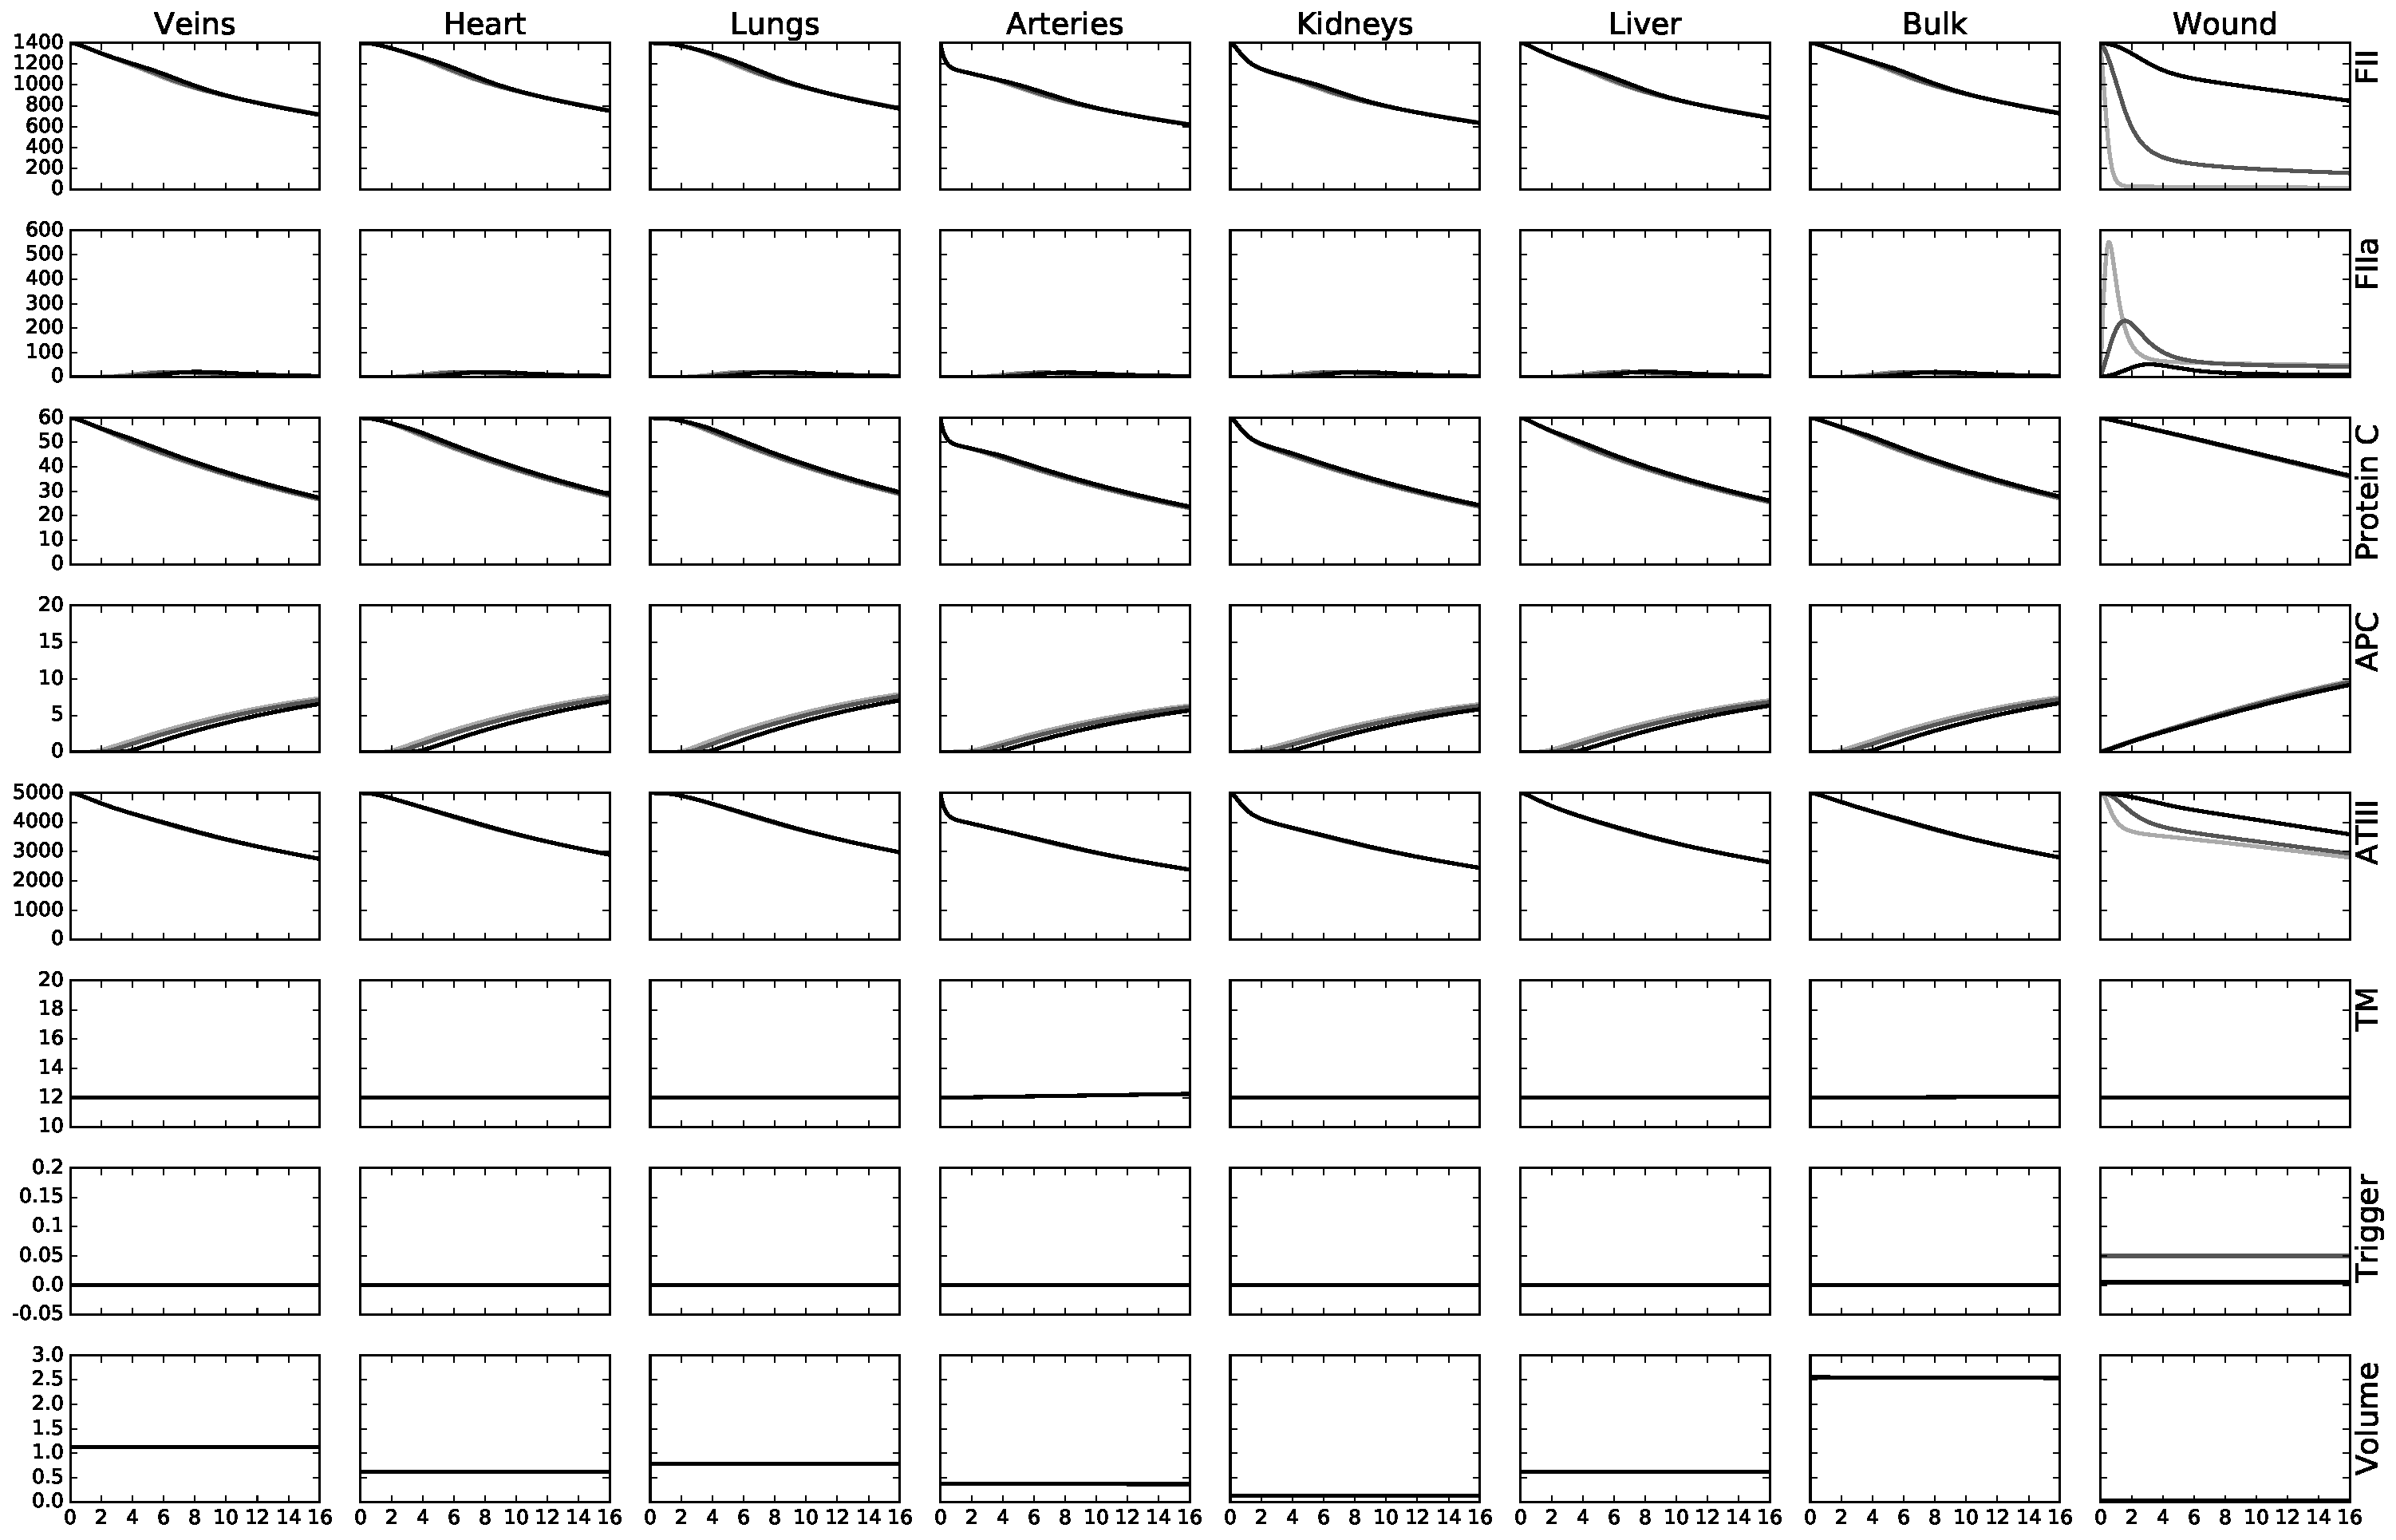
\includegraphics[width=\textwidth]{figures/ComparisonofTriggerValuesNewLayout}
        \caption{\scriptsize All concentrations given in nanomolar, and times in minutes. Volumes are given in liters. Light grey is a trigger concentration of .5 nanomolar, medium grey is .05 nanomolar, and black corresponds to .005 nanomolar. }
        \label{fig:comparsionoftrigger}
%\end{wrapfigure}
\end{figure}
\subsection*{PBPK With Changing Heart Rate and Volume Changes}

There are three phases of hemorrhage. When less than 10\% of blood volume has been lost, the barroreflex kicks in as pressure has dropped to increase heart rate. \cite{foex1999systemic} After approximately 10\% of blood volume has been lost, heart rate because to decrease, as does blood pressure. When blood loss approaches 30\% of blood volume, heart rate increases dramatically.\cite{jacobsen1990cardiovascular} During all three phases, the concentrations of adrenaline, noradrenaline, and vavasopressin rise, but then decrease once blood is transfused.
Using the blood pressure tracks from the MIMIC II numerics data base, we used Olufsen's and Ottsen's model to predict heart rate, and used the predicted heart rate within the PBPK model. \cite{olufsen2013practical} The details of the heart rate prediction model are given in the supplimental material.

\begin{wrapfigure}{L}{.61\textwidth}
        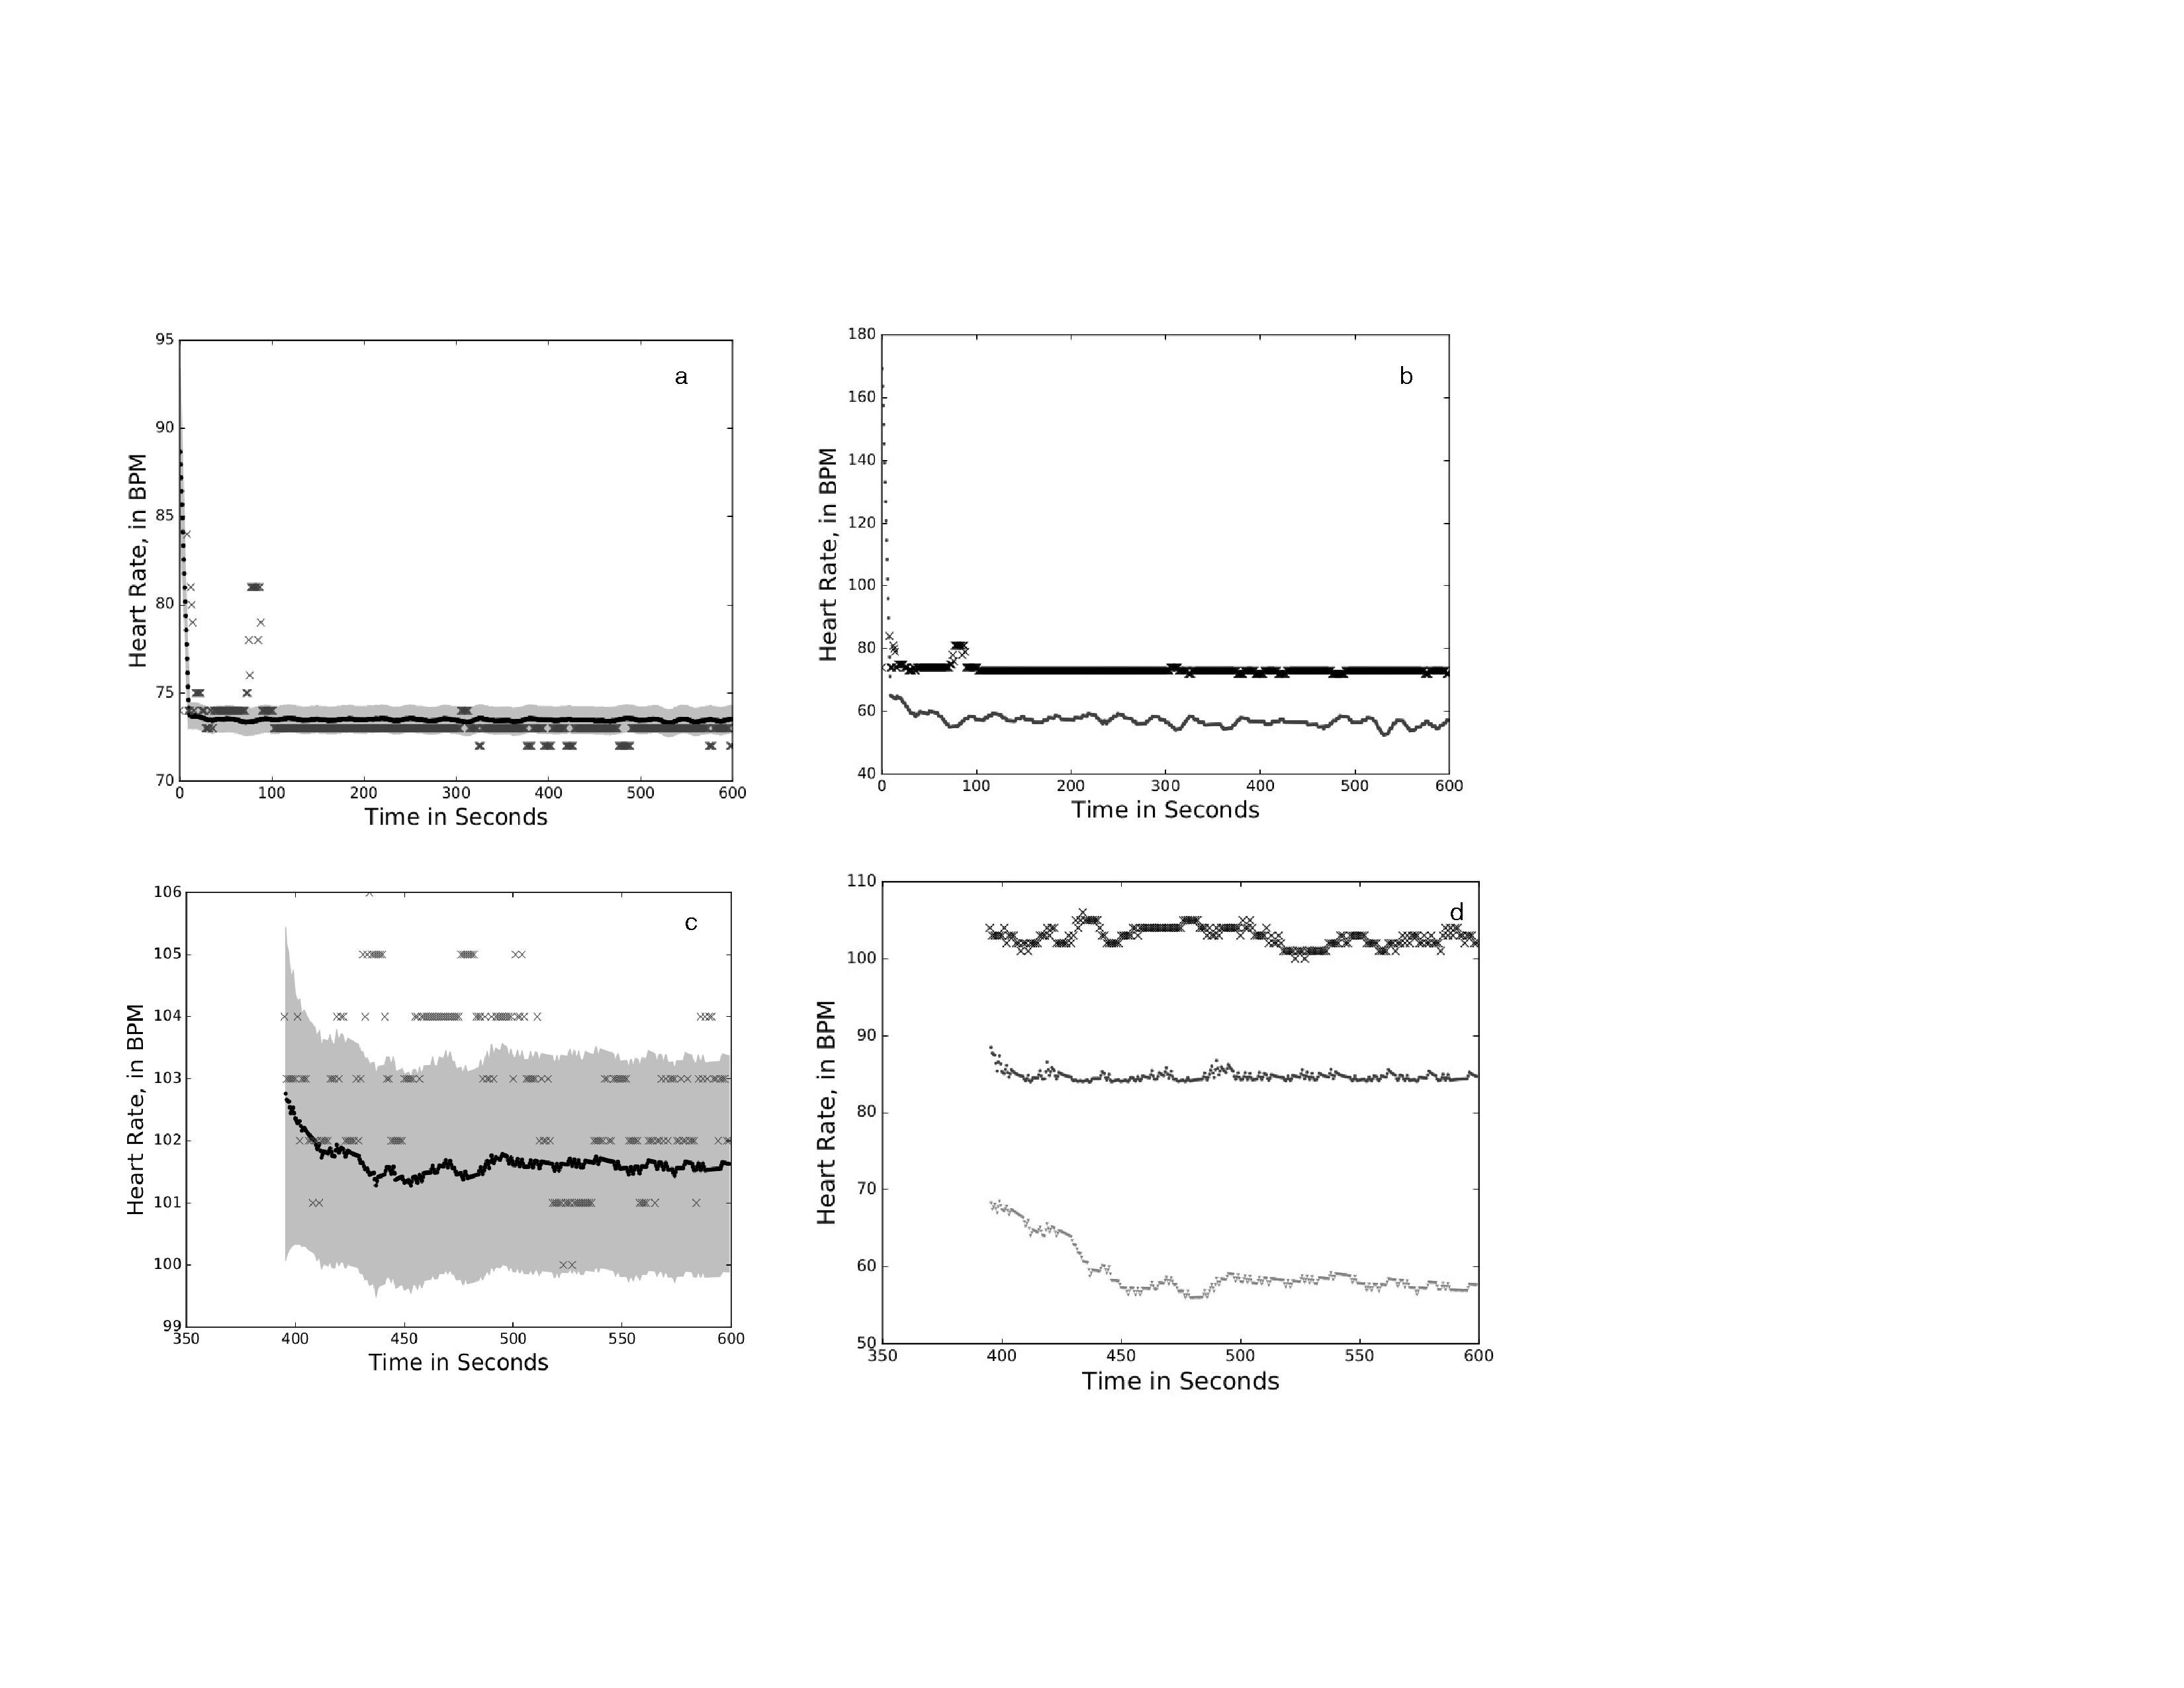
\includegraphics[width=.6\textwidth,trim = {4cm 6cm 15cm 8cm},clip]{figures/singlevsmulti}
         
       \caption{\scriptsize The x represent the true data, the black dots represent the average model performance over the 10 different parameter sets, and the grey is a 95\% confidence interval. Figures a and b are cluster 1 patient, Figures c and d show cluster a 2 patient. The left column uses the parameters estimated by simulated annealing, the right side shows performance of the original parameters in light grey and the parameters estimated by Nelder-Mead in dark grey.}   
       \label{fig:mulitobjperformance}
\end{wrapfigure}

 We used the Nelder Mead algorithm to find a set of parameters that better fit the MIMIC II data to get better agreement between the blood pressure predicted by the model and the recorded blood pressure. Additionally, we used k-means clustering to group the patients into two clusters, based on age, average heart rate, and SAPS (Simplified Acute Physiology) score. We used the JuPOETS package, which performs simulated annealing combined with Pareto optimality to generate families of parameters for the two clusters. \cite{bassen2016jupoets} The performance of the families of parameters on patients on each cluster is shown in \ref{fig:mulitobjperformance}. The estimated parameters reduced the total mean squared error by more than two-thirds. 
 
Furthermore, we used the acetylcholine and noradrenaline concentrations predicted by this model to vasodilate and constrict the arterial and venous blood pools.The aerial and venous blood are constricted if the noradrenaline concentration is above a threshold value, and dilated if the acetylcholine concentration is above a threshold value. The expansion and contraction of the compartments was capped at 125\% and 75\% of their resting values, respectively. The degree of volume change was based on previous experimental data on volume change as a function of a concentration of acetylcholine and noradrenaline.\cite{chowienczyk1994blood} $^,$ \cite{dora1983effect} A comparison of the updated model versus holding the heart rate constant at 100 bpm is shown in Figure \ref{fig:comparsionPBPK}. The slower increase in thrombomodulin (TM) levels in the arteries and bulk is due to the fact that the patient is bleeding out more slowly with the reduced heart rate from the MIMIC II track. In general, all of the curves follow the same trends, although their shape changes slightly when the heart rate changes. The results of peturbing the starting organ volumes and initial concentrations by up to 25\% of their nominal values are shown in the supplimental material. Allowing the concentrations to alter results in a much broader concentration profile than allowing the organ volumes to change.
 \begin{figure}[!htb]
 %\begin{wrapfigure}[22]{R}{\textwidth}
        \centering
        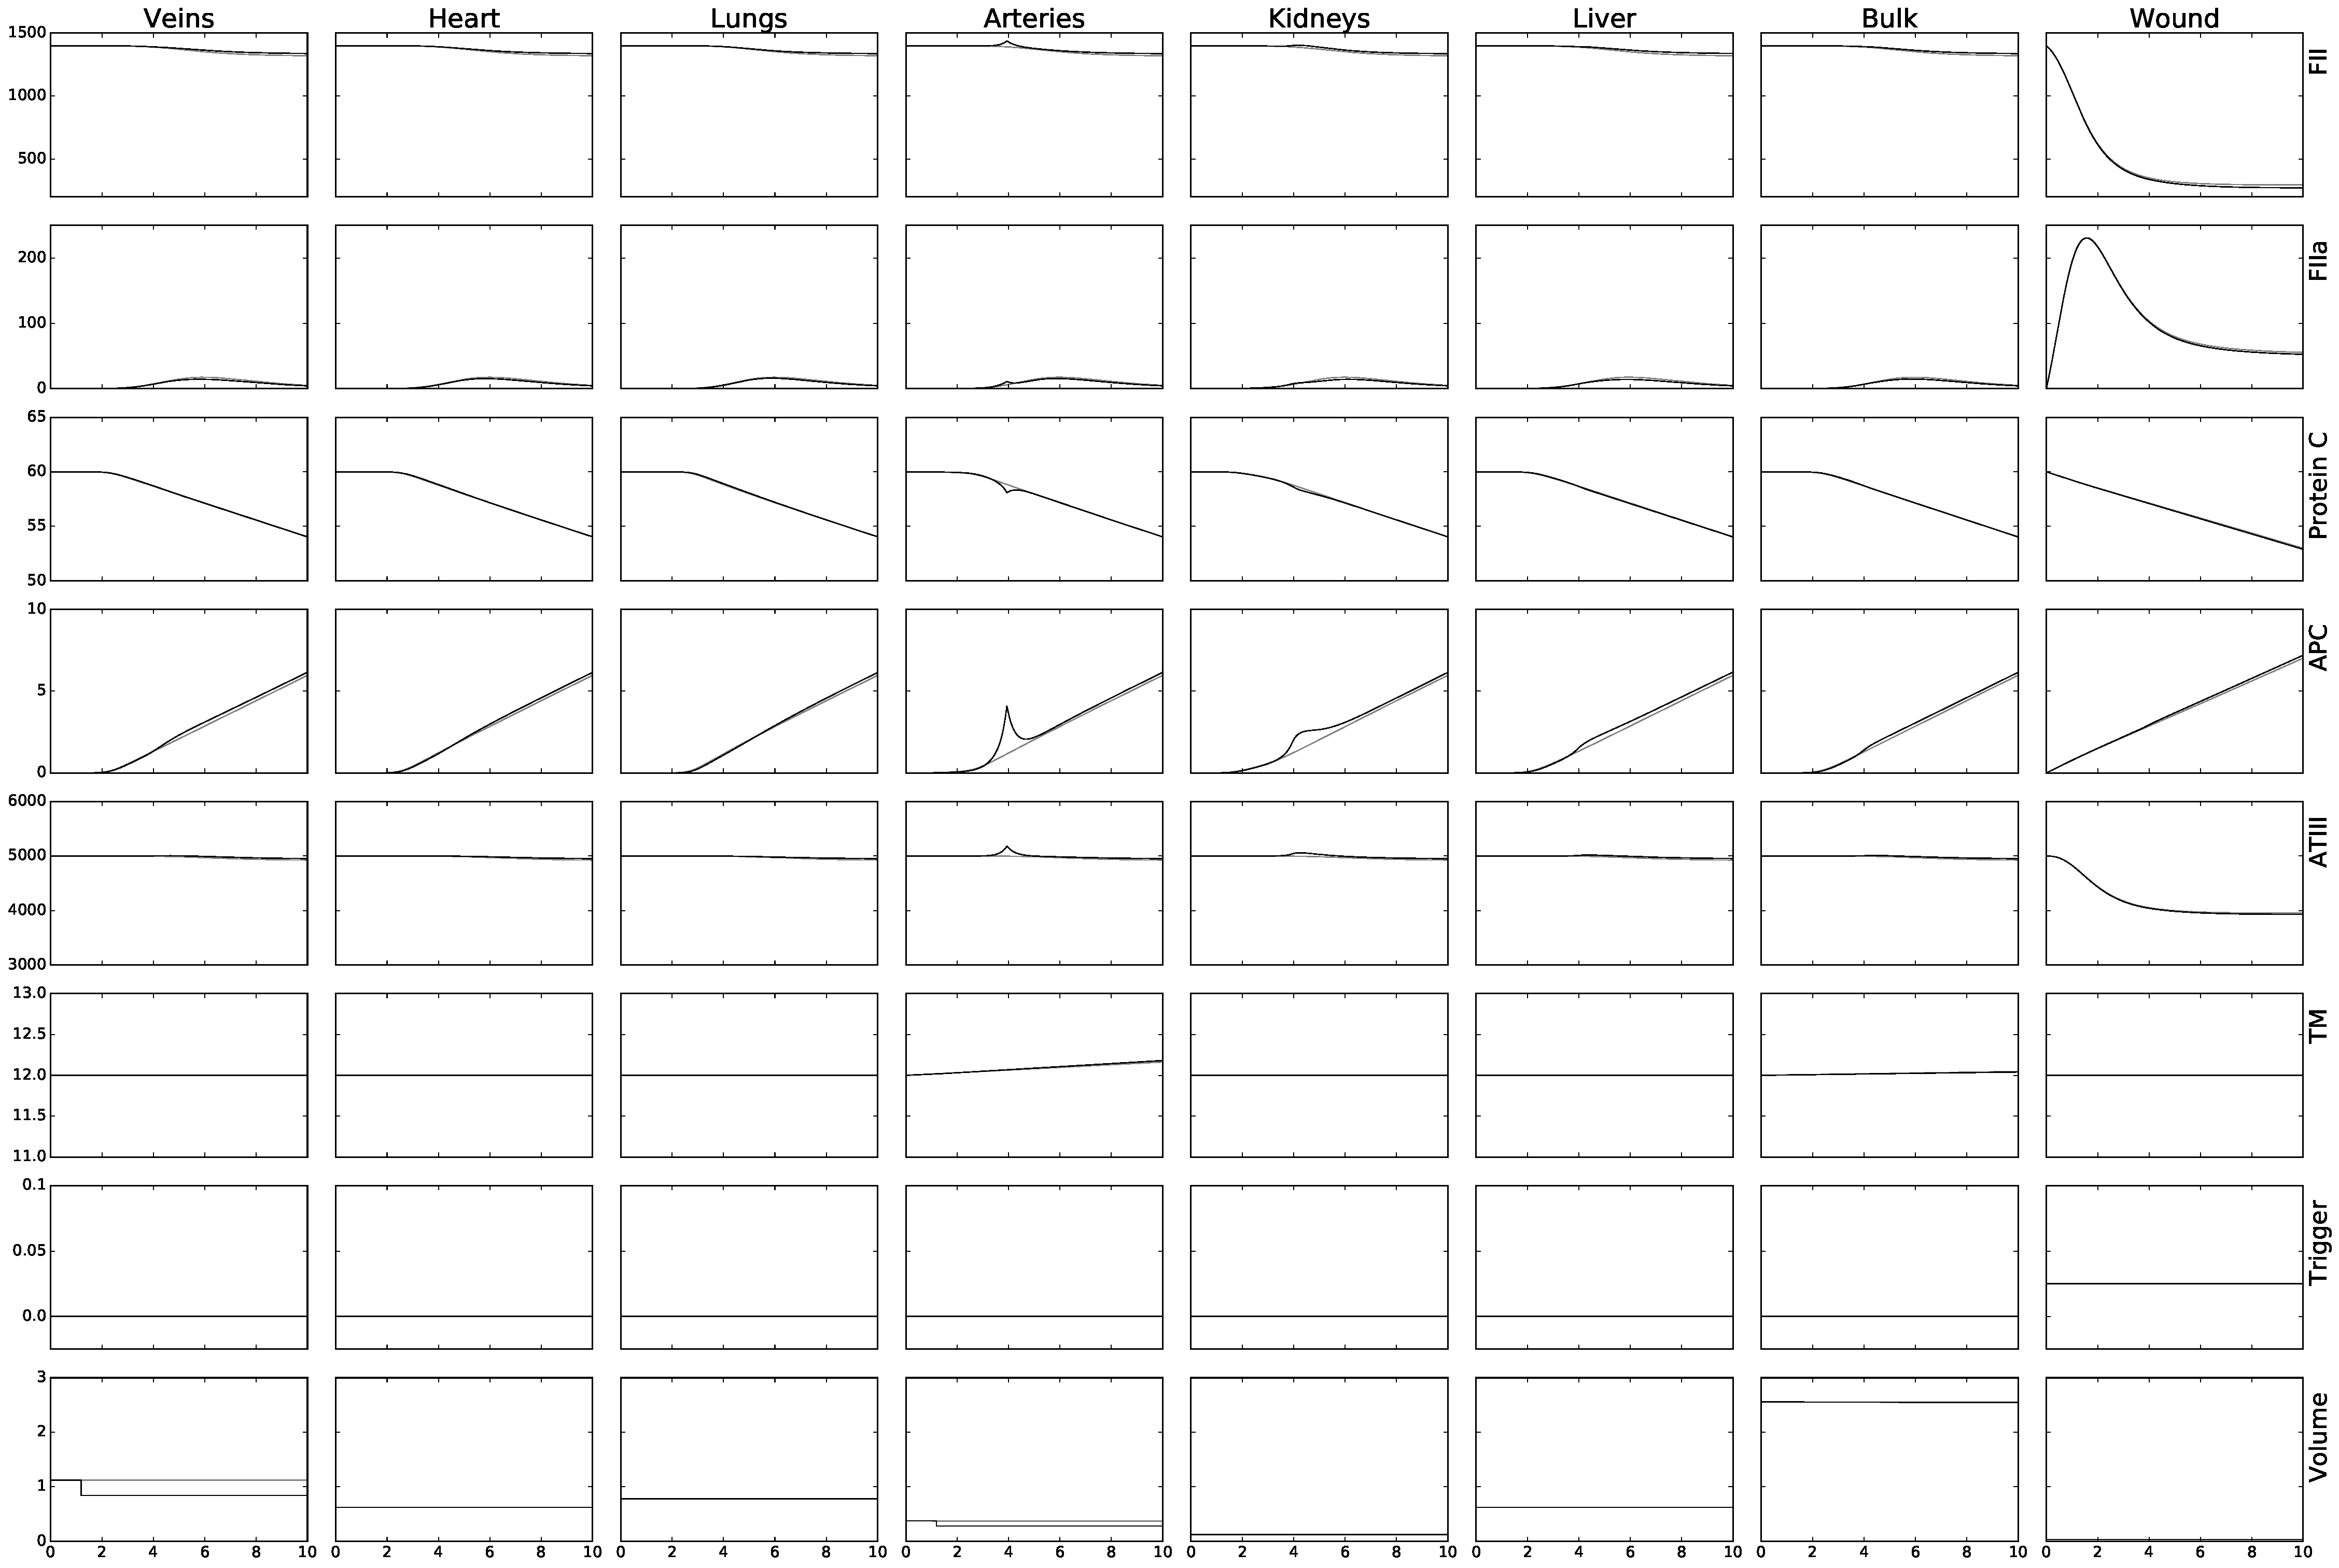
\includegraphics[width=\textwidth]{figures/s31060-2832-03-02-17-54nComparisonGreyConstHRBlackVarryingPPatient}
        \caption{\scriptsize Grey is holding the heart rate constant at 100 bpm, black is allowing the heart rate to varry based on a pressure track (recorded at 1 Hz) of a MIMIC II patient. The spikes shown in black are from compartment changes, due to vasodilation and contraction. Organ blood volumes are based on a 70 kg man, with a total blood volume of 6234 mL.\cite{davy1994total} $^,$ \cite{leggett1991suggested}}
        \label{fig:comparsionPBPK}
%\end{wrapfigure}
\end{figure}


 
\newpage
\section*{Research Plan}
\subsection*{Incorporate pH Change in Body Model}
The activities of the proteins involved in coagulation are highly pH sensitive, and acidosis is another leg of the ``lethal triad". The activity of FVIIa is reduced by 90\% when the blood's pH is lowered from its normal value of 7.4 to 7.0, and the activity of the FVIIa/tissue factor complex is reduced by 60\%. \cite{meng2003effect} To accurately model coagulation in a holistic manner, this effect should be taken into account.
\subsection*{Hepatic Injury}
Many of the proteins involved in coagulation and fibrinolysis are synthesized in the liver. If it is damaged, the replacement rates of these proteins will be altered. Patients suffering from acute liver injury tend to have depressed concentrations of FII, FV, FVII, FXI and FX, and elevated concentrations of FVIII. \cite{kerr2003effects} 
\subsection*{Model Fluid Inputs}
Trauma patients are generally given fluids intravenously to prevent shock, maintain blood pressure and reduce tissue damage, however, there is no clear evidence supporting a certain dosage or schedule for intravenous fluids. \cite{kwan2014timing} $^,$ \cite{roberts2001normalisation} The types of fluids, and at what ratio they should be given is still a matter of study. \cite{spahn2007management} 
\subsection*{Model Effects of Transexamic Acid}
Transexamic acid, a lysine derivative, acts to prevent fibrinoylsis by blocking lysine binding sites on plasmiogen.\cite{dunn1999tranexamic} The CRASH-2 study showed that administering transexamic acid within one hour of injury reduced mortality from bleeding by 32\%, but increases mortality if the drug is administered more than three hours after injury.\cite{crash2011importance} The mechanism leading to increased mortality after delayed administration of transexamic acid is not clear, and can be investigated by my model, as well as the ideal dosing schedule. 
\subsection*{Incorporate Fibrinolysis Model}
A reduced order model of fibrinolysis is currently under development by the Varner group. This model expands on the reduced order coagulation model by including 18 species. Incorporating it into PBPK will allow us to study both coagulopathy and DIC. 
\subsection*{Personalization}
In an ideal case, we could instantaneously sequence the DNA of the individual and predict how they will respond to various treatments, but science has not yet advanced to that level. Humans are not identical-they have differing masses and body compositions. Additionally, people respond differently to the same drug dosage, owing to their different compositions and gene expression levels.  
Studies have been done to link genes to coagulation disorders  and to correlated genes with activated partial thromboplastin time and prothombin time.\cite{soria2009genetic}$^,$\cite{tang2012genetic} If genetic information is available about a patient, we can use this information to alter the dynamics of coagulation within the PBPK to better predict outcomes.
Correlations exist for blood volume as a function of weight, for both men and women, as do estimates of the blood contained by various organs. \cite{feldschuh1977prediction}$^,$\cite{leggett1991suggested}The P$^3$M project has developed a large set of bodies that can be used to test PBPK models. \cite{price2003modeling} This set of bodies includes both organ masses as well as perfusion rates. We can use this spectrum of bodies to see compare coagulation and fibrinolysis in bodies of varying size and composition. 
\newpage
%%%%%%%%%%%%%%%%%%%%%%%%%%%%%%%%%%%%%%%%%%%%%%%%%%%%%%%%%%%%%%%%%%%%%
% OTHER STUFF
%%%%%%%%%%%%%%%%%%%%%%%%%%%%%%%%%%%%%%%%%%%%%%%%%%%%%%%%%%%%%%%%%%%%%
%%%%%%%%%%%%%%%%%%%%%%%%%%%%%%%%%%%%%%%%%%%%%%%%%%%%%%%%%%%%%%%%%%%%%
% BIBLIOGRAPHY
%%%%%%%%%%%%%%%%%%%%%%%%%%%%%%%%%%%%%%%%%%%%%%%%%%%%%%%%%%%%%%%%%%%%%
\bibliography{lecover-q-ref}
\bibliographystyle{ieeetr}
\pagebreak
%%%%%%%%%%%%%%%%%%%%%%%%%%%%%%%%%%%%%%%%%%%%%%%%%%%%%%%%%%%%%%%%%%%%%
% Fig.S
%%%%%%%%%%%%%%%%%%%%%%%%%%%%%%%%%%%%%%%%%%%%%%%%%%%%%%%%%%%%%%%%%%%%%
\beginsupplement
\section*{Supplimental Material}
\begin{figure}[H]
        \centering
        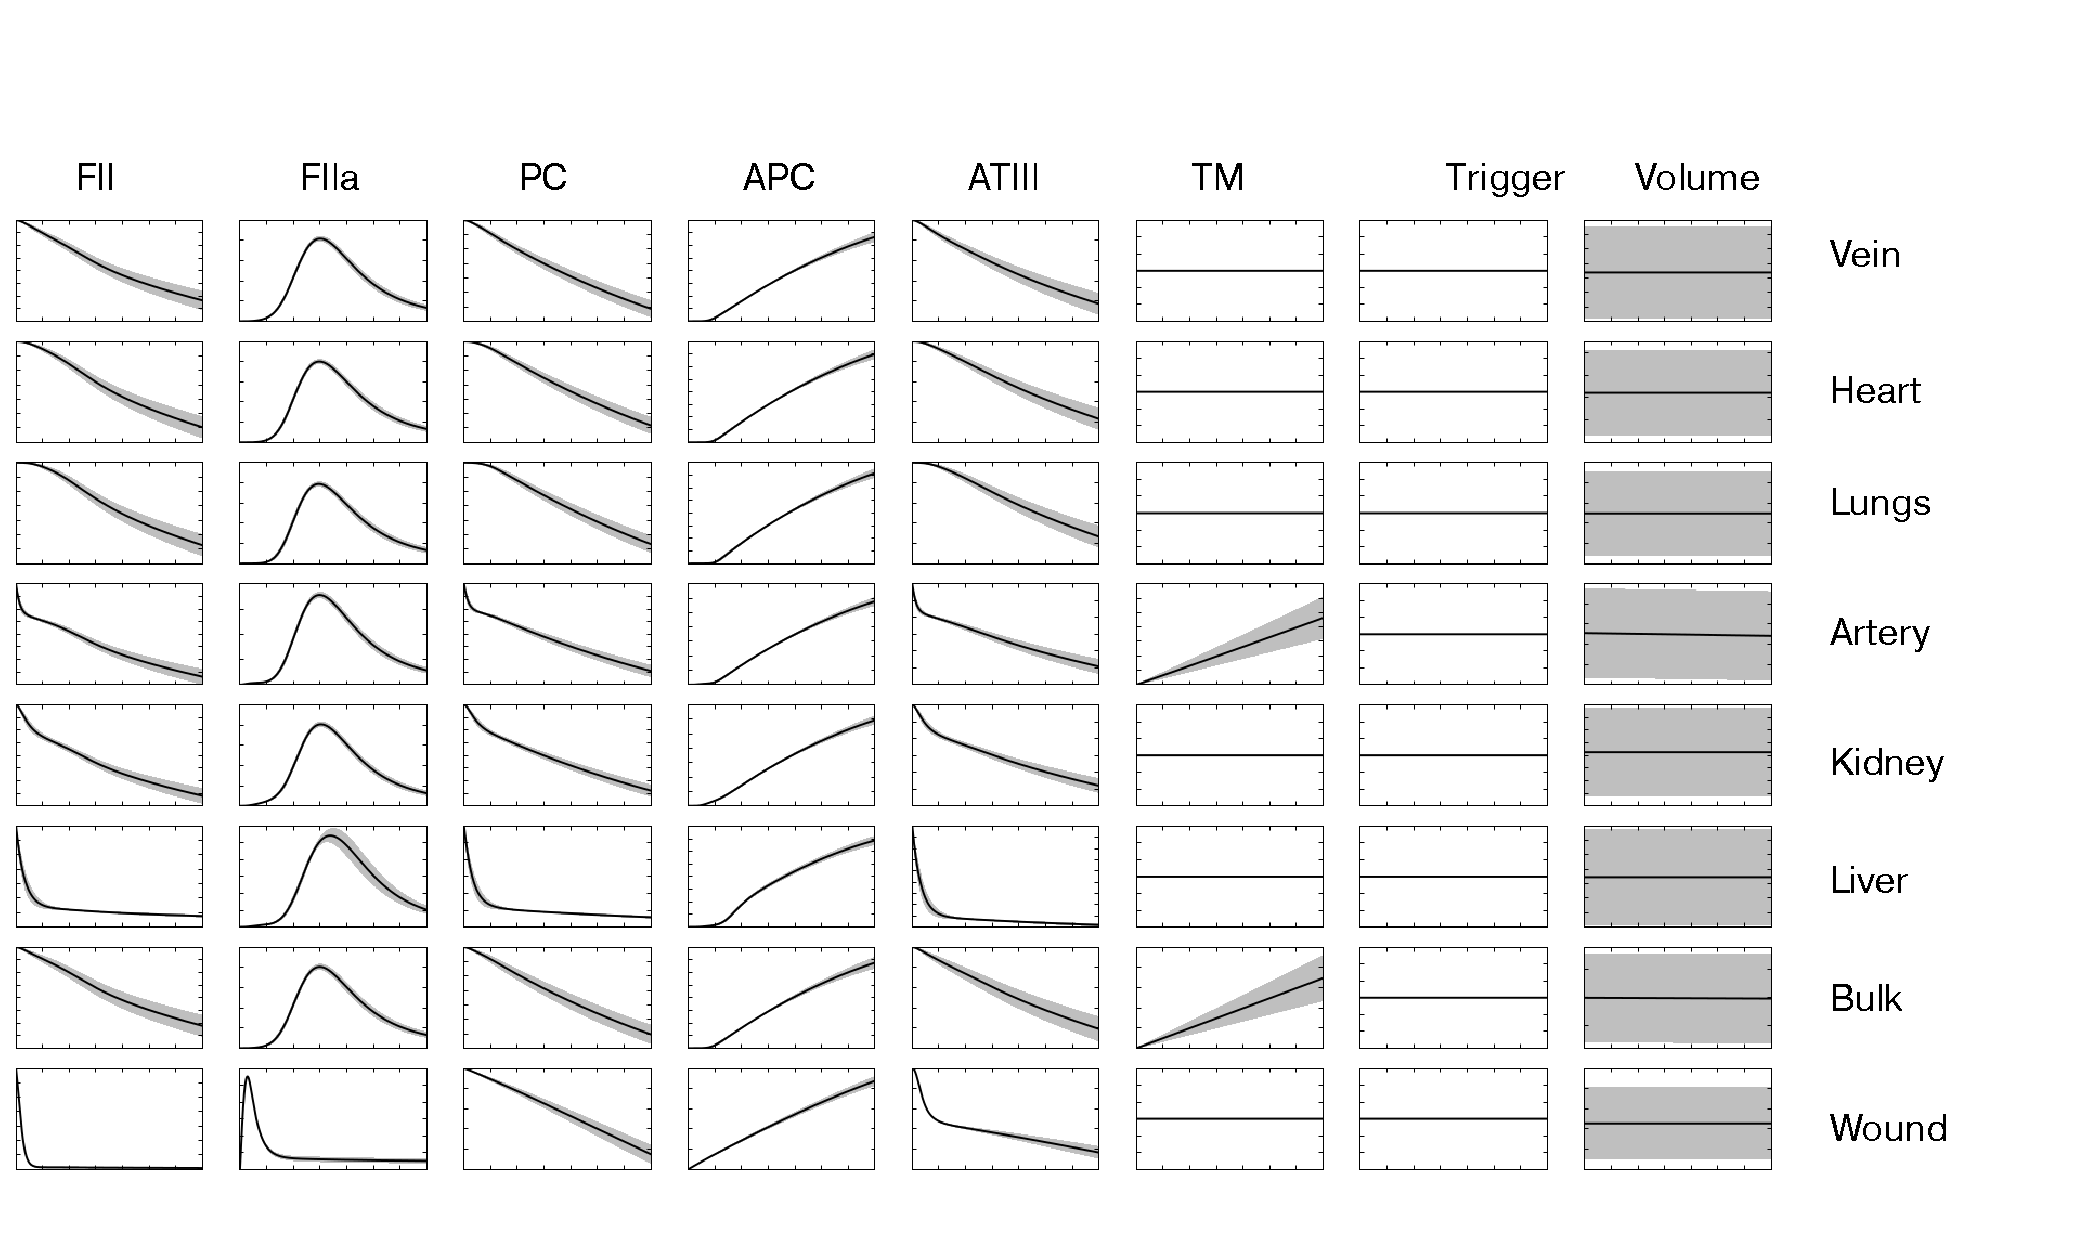
\includegraphics[width=\textwidth]{figures/DifferingInitialVolumesPretty}
        \caption{\scriptsize Black is the mean value for 100 patients, grey shows the 95\% confidence interval.Initial concentrations in each compartment were permitted to alter up to 25\% of their nomial value.}
        \label{fig:peturbOrganVolumes}
\end{figure}

\begin{figure}[H]
%\begin{wrapfigure}{R}{\textwidth}
        \centering
        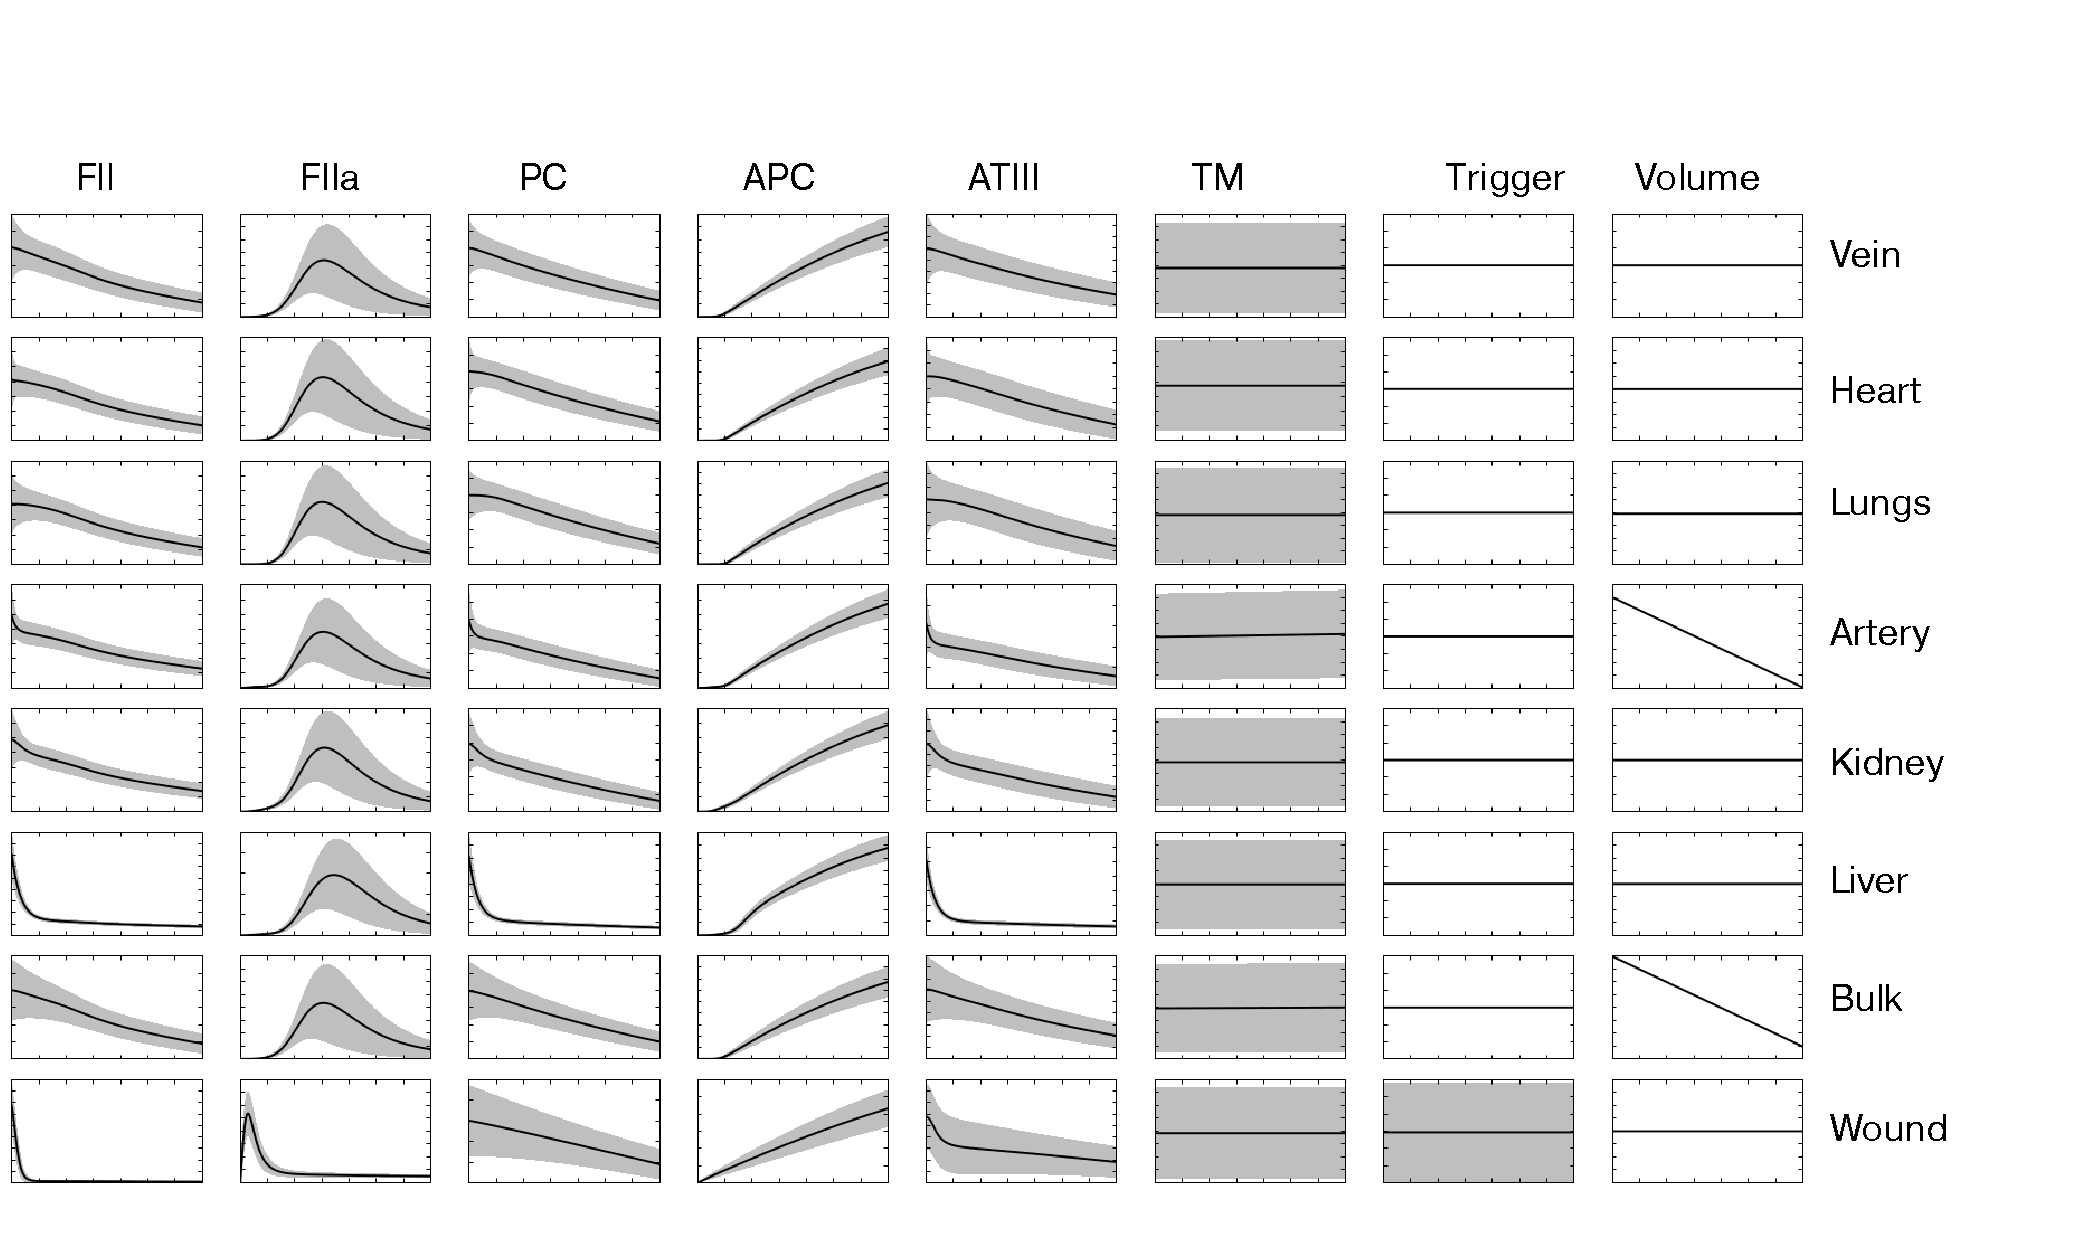
\includegraphics[width=\textwidth]{figures/DifferingInitialConcentrationsPretty}
        \caption{\scriptsize Black is the mean value for 100 patients, grey shows the 95\% confidence interval. Initial concentrations in each compartment were permitted to alter up to 25\% of their nomial value.}
        \label{fig:peturbOrganVolumes}
%\end{wrapfigure}
\end{figure}

\subsection*{Heart Rate Prediction Model}
The rate at which a heart beats is determined, in part, by the sympathetic and parasympathetic portions of the nervous system. When the sympathetic nervous system is stimulated, it releases epinephrine and norepinephrine  which increase heart rate. The parasympathetic system releases acetylcholine which decreases heart rate.  These two systems, often described as an accelerator and a brake, are not totally independent on each other, rather, they interact through second messengers cAMP and cGMP. \citep{olshansky2008parasympathetic}
Heart rate is also controlled by the baroreflex system. The baroreflex system consists of baroreceptors, tension sensitive nerve endings found in the circulatory system. \citep{ottesen1997modelling} When they sense a change in pressure, they cause a change in the frequency of nerve activity. When pressure (and stretch) rapidly increase, so does the baroreceptor firing rate. \citep{negative1999reflexes} This effects of this signal are not instantaneous, rather, there is a time delay on the order of seconds before the sympathetic and parasympathetic nervous systems respond. \citep{ottesen1997modelling}
Olufsen and Ottesen have developed models of heart rate based on blood pressure measurements.\citep{olufsen2013practical} These models use the baroreflex system and the concentrations of acetylcholine and n to predict heart rate. In their models, they assume that they changes in arterial wall stretch are proportionate to filtered blood pressure such that
\begin{equation}
\bar p = \int_{-\infty}^{t} p(s)e^{-\alpha(t-s)}ds
\end{equation}
or, equivalently, 
\begin{equation}
\frac{d \bar p}{dt} = \alpha(-\bar p + p)
\end{equation}
where $\alpha$ is a gain, $\bar p$ is the filtered blood pressure, and $p$ is the patient's measured blood pressure. 
From $\bar p$, we can predict the nervous system firing rate, $n$
\begin{equation}
n = \sum_i n_i + N, i = 1,2
\end{equation}
where N is a baseline firing rate and $n_i$ correspond to the firing rates of nerve fibers of type $i$. The firing rates for nerves of type $i$ are computed as
\begin{equation}
\frac{dn_i}{dt} = \kappa_i \frac{d \bar p}{dt} \frac{n(M-n)}{(M/2)^2}-\frac{n_i}{\tau_i}, i = 1,2
\end{equation}
where $M$ is the maximum firing rate, and $\tau_i$ is the time scale for nerves of type $i$. 
The firing rate information is compiled by the central nervous system, which then determines the the sympathetic and parasympathetic outputs, $f_{sym}$ and $f_{par}$, respectively. 
\begin{equation}
f_{par} = n/M
\end{equation}
\begin{equation}
f_{sym} = \frac{1-n(t-\tau_d)/M}{1+\beta f_{par}}
\end{equation}
With these outputs, we can determine the dimensionless concentrations of acetylcholine, $c_{ach}$ and noradrenaline, $c_{nor}$
\begin{equation}
\label{dcnordt}
\frac{dc_{nor}}{dt} = \frac{f_{sym}-c_{nor}}{\tau_{nor}}
\end{equation}
\begin{equation}
\label{dcachdt}
\frac{dc_{ach}}{dt} = \frac{f_{par}-c_{ach}}{\tau_{ach}}
\end{equation}
where each $\tau$ represents a time scale. 
Finally, we can calculate the heart rate, from $h_0$, the intrinsic heart rate, and $m_{nor}$ and $m_{ach}$, which are weights for the contributions of acetylcholine and norepinephrine  to heart rate in the form
\begin{equation}
\label{h}
h = h_0(1+m_{nor}c_{nor} - m_{ach}c_{ach})
\end{equation}
The above equations are from Olufsen and Ottesens 2011 paper, however, they have published many other models with similar forms.\citep{olufsen2006modeling} $^,$ \citep{ottesen1997modelling} $^,$ \citep{olufsen2008modeling} This model was selected because of the small number of parameters compared to other models. We solved this system of linked differential equations using the ode23s and ode78 functions of the Julia language ODE package. 
\end{document}
